\documentclass{book}

\usepackage{gensymb}
\usepackage{graphicx}
\usepackage[hidelinks]{hyperref}
\hypersetup{
	linktoc=all
}
\usepackage{siunitx}
\usepackage{textgreek}

\begin{document}
\title{Vitamins}
\author{Radu-Mihai Rotariu}
\maketitle
\pagenumbering{roman}
\tableofcontents\newpage
\pagenumbering{arabic}

\chapter{Vitamin A}
\begin{figure}[h]
	\caption{Chemical structure of Retinol}
	\centering 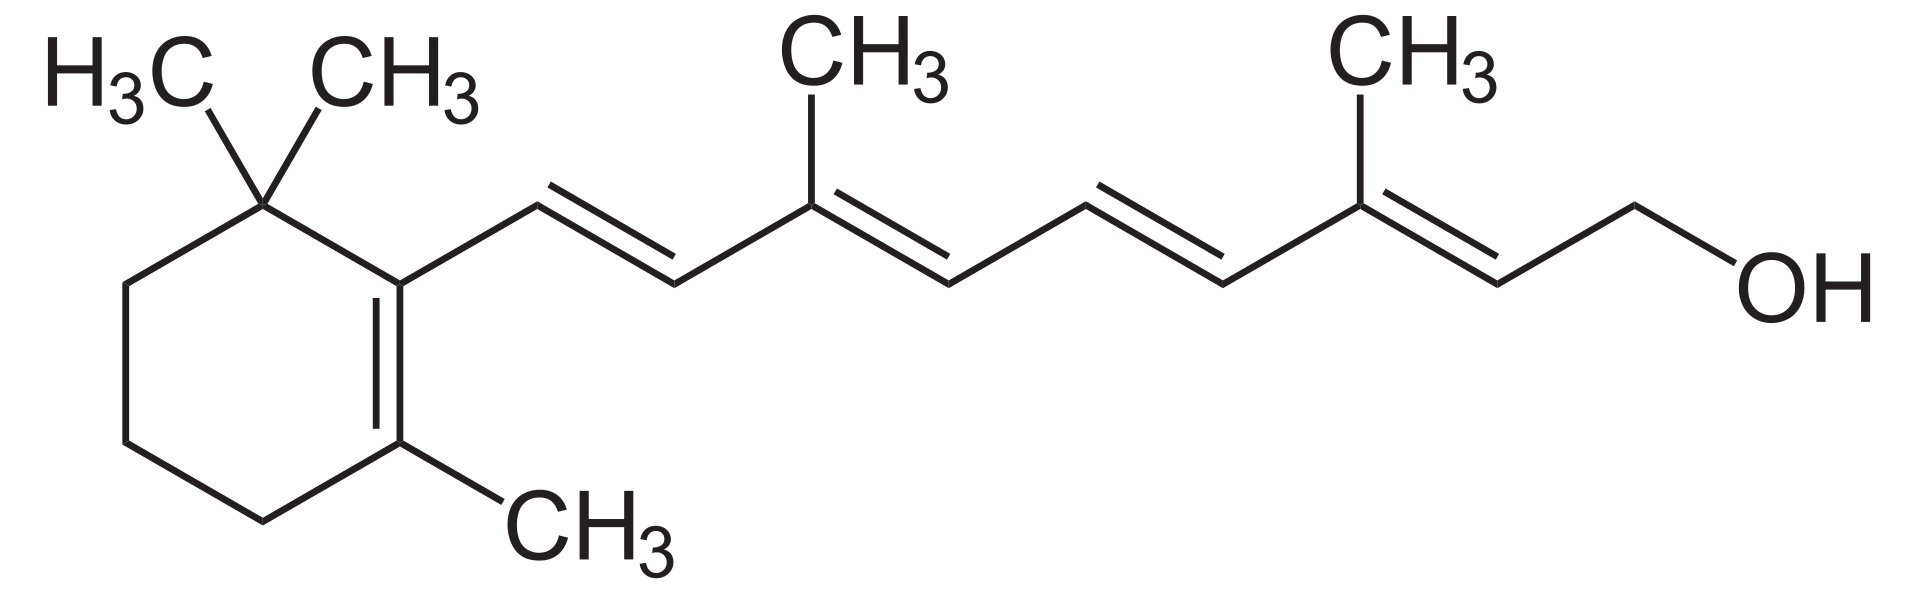
\includegraphics[width=\textwidth]{images/Vitamin_A_chemical_structure}
\end{figure}

\begin{table}[h]
	\caption{Chemical and physical data}
	\centering \begin{tabular}{| r | l |}
		\hline
		Formula & C\textsubscript{20}H\textsubscript{30}O\\ \hline
		Molar mass & 286.459 g$\cdot$mol \textsuperscript{-1}\\ \hline
		SMILES & OC/C=C(C)/C=C/C=C(C)/C=C/C1=C(C)/CCCC1(C)C\\ \hline
	\end{tabular}
\end{table}
\newpage

\section{About}
Vitamin A is a fat-soluble vitamin and essential nutrient. The term itself refers to a family of compounds, which includes: retinol, retinal (also known as retinaldehyde), retinoic acid, and provitamin carotenoids (precursors), most notable being \textbeta-carotene.

Vitamin A is found in food in two forms:
\begin{itemize}
	\item Retinol, found in animal-sourced foods, either as retinol or bound to a fatty acid to become a retinyl ester.
	\item Carotenoids \textalpha-carotene, \textbeta-carotene, \textgamma-carotene, and the xanthophyll \textbeta-cryptoxanthin. All of these carotenoids function as precursors to vitamin A in herbivores and omnivores which possess the required cleaving enzymes needed to convert the carotenoids to retinal and then the retinal to retinol. Some carnivore animals lack this enzyme. All the other carotenoids have no vitamin activity.
\end{itemize}

\section{Measurement unit}
The agreed upon standard measurement unit is 1\textmu g, which is $\sim$0.33 nmol of retinol. It's also referred to as a \textmu g RAE (Retinol Activity Equivalent).

Since four of the carotenoids can be converted into retinol, an equivalency has been established between the standard measurement unit for retinol and each of the precursors.

As such, here is a list of the standard units of measurements for retinol and its equivalent for all the precursors:

\begin{table}[h]
	\caption{VItamin A standard measurement units}
	\centering \begin{tabular}{| l | c |}
		\hline
		\textbf{Substance and its chemical environment (per 1\textmu g)} & \textbf{\textmu g RAE}\\ \hline
		Retinol & 1\\ \hline
		\textbeta -Carotene, dissolved in oil & 1/2\\ \hline
		\textbeta -Carotene, dietary* & 1/12\\ \hline
		\textalpha -Carotene, dietary* &\\
		\textgamma -Carotene, dietary*& 1/24\\
		\textbeta -Cryptoxanthin, dietary* &\\ \hline
	\end{tabular}
\end{table}

* --- as found in food sources
\newpage

\section{Dietary recommendations}
Listed below are the recommendations from the US National Academy of Medicine. Data summarized from \href{https://nap.nationalacademies.org/read/10026/chapter/6}{\textit{this document}}.

The acronyms used are:
\begin{itemize}
	\item RDA --- Recommended Dietary Allowance
	\item AI --- Adequate Intake
	\item UL --- Upper Limit
\end{itemize}

\begin{table}[h]
	\caption{Retinol Daily Reference Intakes}
	\centering \begin{tabular}{| r | l | l |}
		\hline
		\textbf{Life stage group} & \textbf{RDA or AI (\textmu g RAE/day)} & \textbf{UL (\textmu g RAE/day)}\\ \hline
		Infants (0--6 months) & 400 (AI) & 600\\ \hline
		Infants (7--12 months) & 500 (AI) & 600\\ \hline
		Children (1--3 years) & 300 & 600\\ \hline
		Children (4--8 years) & 400 & 900\\ \hline
		Males (9--13 years) & 600 & 1700\\ \hline
		Males (14--18 years) & 900 & 2800\\ \hline
		Males (\textgreater19 years) & 900 & 3000\\ \hline
		Females (9--13 years) & 600 & 1700\\ \hline
		Females (14--18 years) & 700 & 2800\\ \hline
		Females (\textgreater19 years) & 700 & 3000\\ \hline
		Pregnancy (\textless19 years) & 750 & 2800\\ \hline
		Pregnancy (\textgreater19 years) & 770 & 3000\\ \hline
		Lactation (\textless19 years) & 1200 & 2800\\ \hline
		Lactation (\textgreater19 years) & 1300 & 3000\\ \hline
	\end{tabular}
\end{table}
\newpage

\section{Sources}


\chapter{Vitamin B\textsubscript{1}}
\begin{figure}[h]
	\caption{Chemical structure of  the thiamine cation}
	\centering 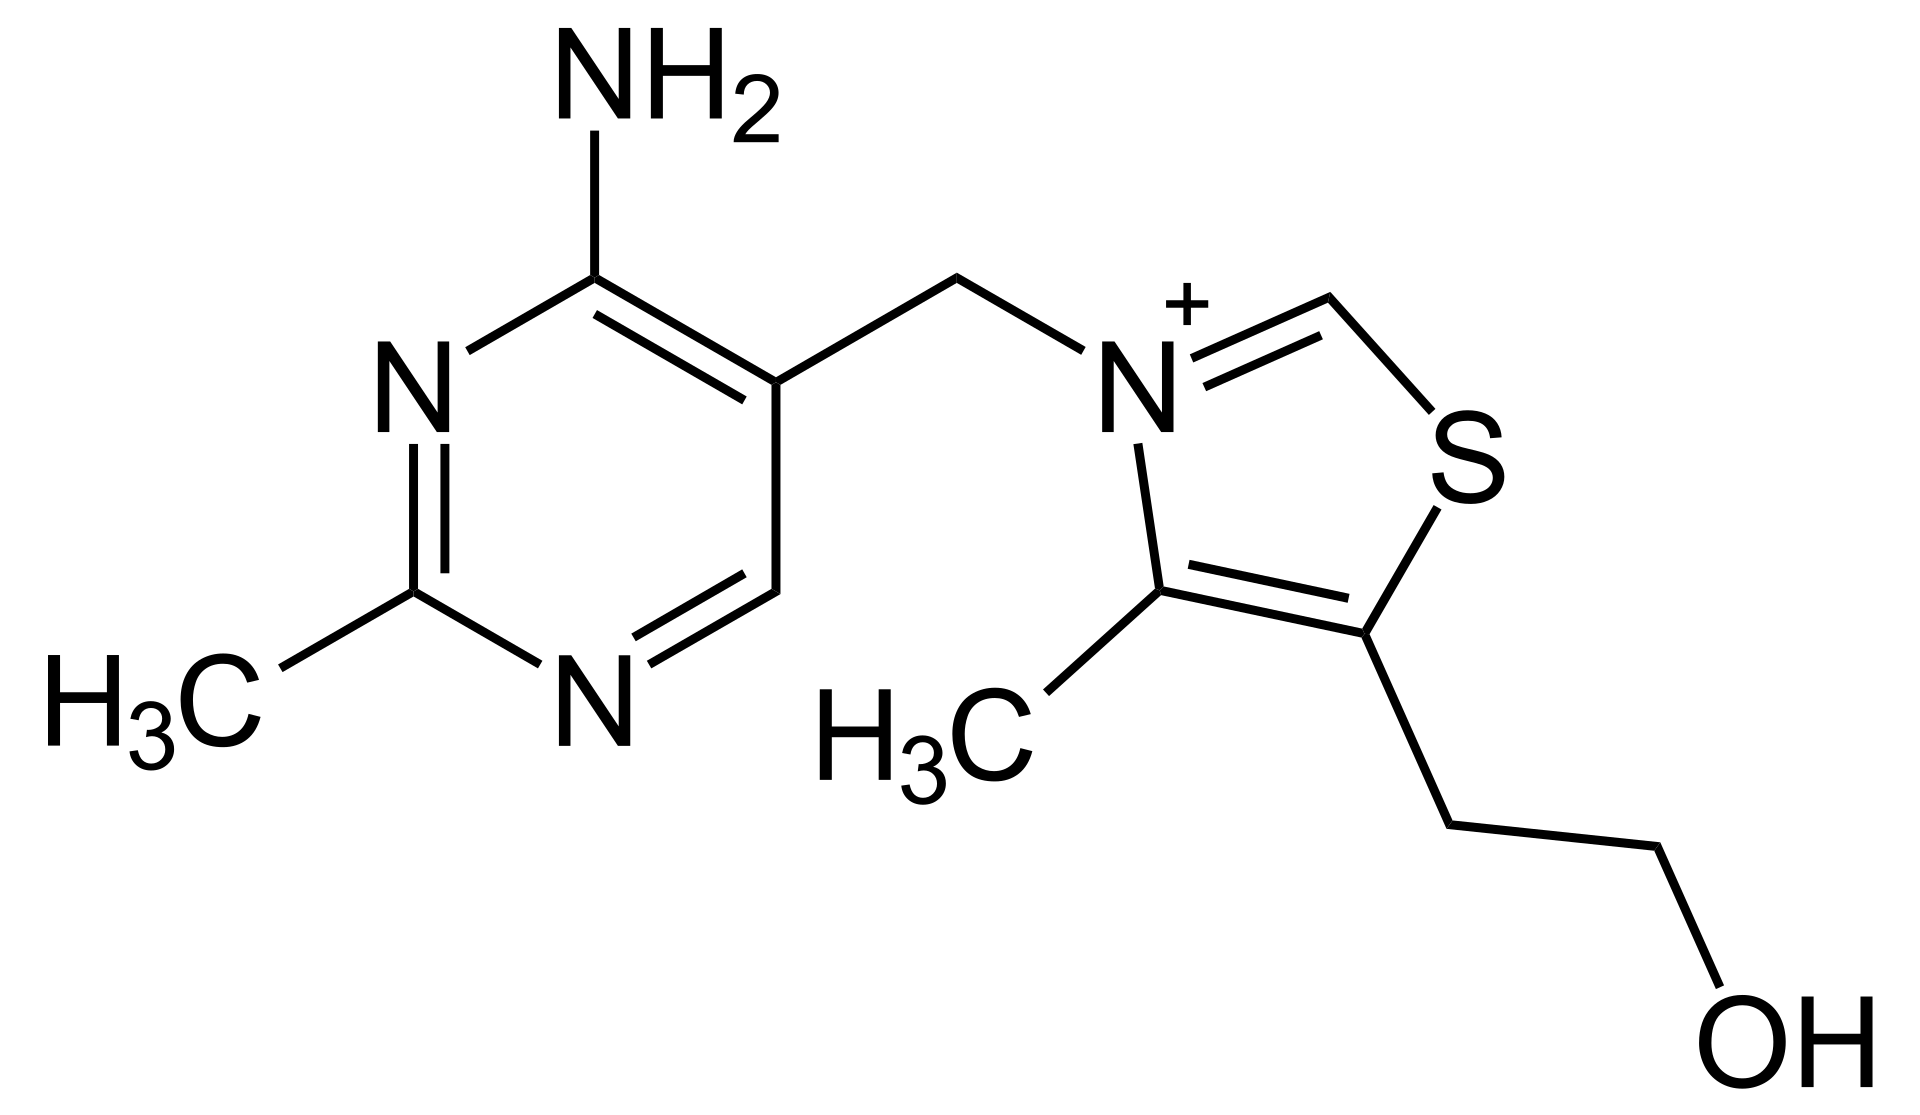
\includegraphics[width=0.75\textwidth]{images/Vitamin_B1_chemical_structure}
\end{figure}

\begin{table}[h]
	\caption{Chemical and physical data}
	\centering \begin{tabular}{| r | l |}
		\hline
		Formula & C\textsubscript{12}H\textsubscript{17}N\textsubscript{4}OS\textsuperscript{+}\\ \hline
		Molar mass & 265.36 g$\cdot$mol \textsuperscript{-1}\\ \hline
		SMILES & Cc2ncc(C[n+]1csc(CCO)c1C)c(N)n2\\ \hline
	\end{tabular}
\end{table}
\newpage

\section{About}
Vitamin B\textsubscript{1}, also known as thiamine or thiamin, is an essential micronutrient that is water soluble.

It is a cation and usually it is supplied as a chloride salt. In the body the most well known and studied derivative of it is TPP (thiamine pyrophosphate), which is a coenzyme used in the catabolism of sugars and amino acids.

\section{Dietary recommendations}
Listed below are the recommendations from the US National Academy of Medicine. Data summarized from \href{https://nap.nationalacademies.org/read/6015/chapter/6}{\textit{this document}}.

The acronyms used are:
\begin{itemize}
	\item RDA --- Recommended Dietary Allowance
	\item UL --- Upper Limits
\end{itemize}

\textbf{Note}: Neither the US National Academy of Medicine nor the European Food Safety Authority have determined the tolerable upper intake level for thiamine.

\begin{table}[h]
	\caption{Vitamin B\textsubscript{1} Daily Reference Intakes}
	\centering \begin{tabular}{| r | l | l |}
		\hline
		\textbf{Life stage group} & \textbf{RDA (mg/day)} & \textbf{UL (mg/day)}\\ \hline
		Infants (0--6 months) & 0.2 & unknown\\ \hline
		Infants (7--12 months) & 0.3 & unknown\\ \hline
		Children (1--3 years) & 0.5 & unknown\\ \hline
		Children (4--8 years) & 0.6 & unknown\\ \hline
		Children (9--13 years) & 0.9 & unknown\\ \hline
		Females (14--18 years) & 1.0 & unknown\\ \hline
		Males (\textgreater14 years) & 1.2 & unknown\\ \hline
		Females (\textgreater19 years) & 1.1 & unknown\\ \hline
		Pregnant/lactating females (14--50 years) & 1.4 & unknown\\ \hline
	\end{tabular}
\end{table}
\newpage

\section{Sources}


\chapter{Vitamin B2}
\begin{figure}[h]
	\caption{Chemical structure of Vitamin B2}
	\centering 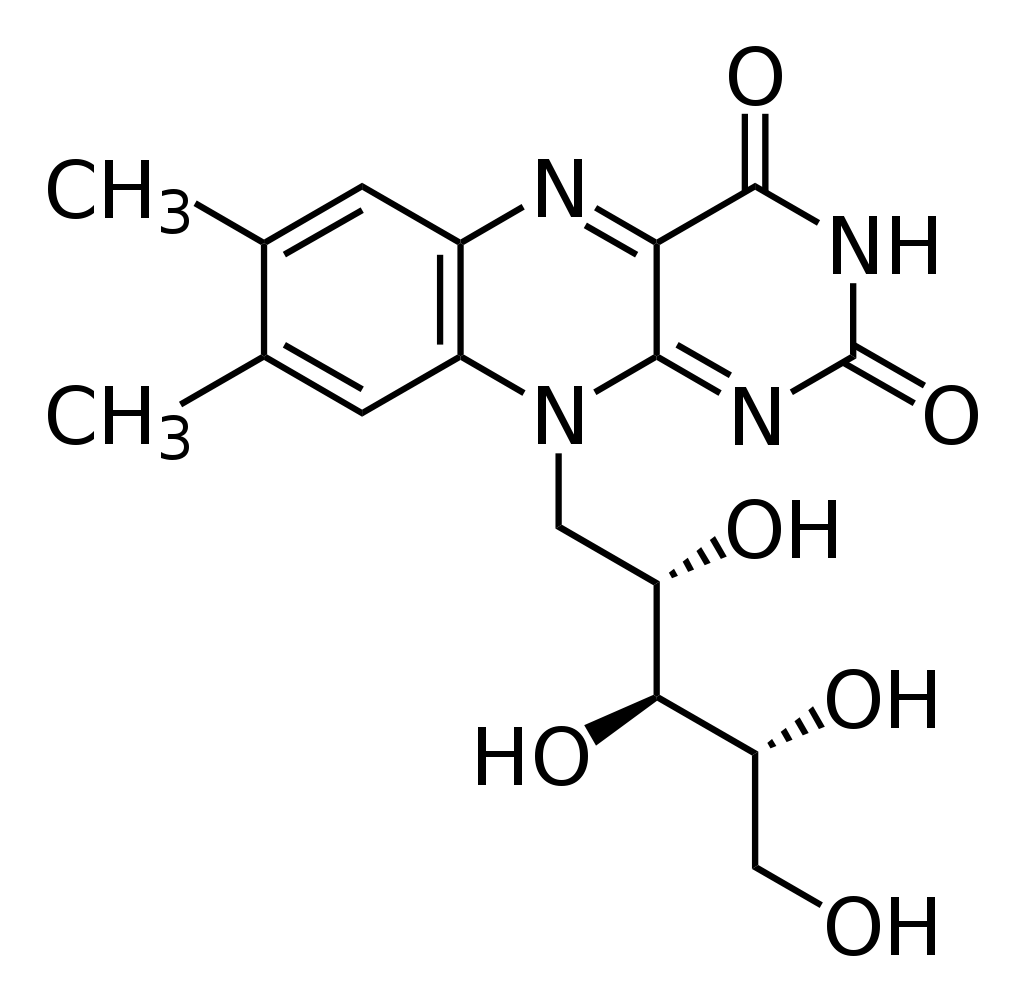
\includegraphics[width=0.5\textwidth]{images/Vitamin_B2_chemical_structure}
\end{figure}

\begin{table}[h]
	\caption{Chemical and physical data}
	\centering \begin{tabular}{| r | l |}
		\hline
		Formula & Smt\\ \hline
		Molar mass & X g$\cdot$mol \textsuperscript{-1}\\ \hline
		Melting point & A--B \degree C (X--Y \degree F)\\ \hline
		Boiling point & A--B \degree C (X--Y \degree F)\\ \hline
		SMILES & \\ \hline
	\end{tabular}
\end{table}
\newpage

\section{About}


\section{Measurement unit}


\section{Dietary recommendations}


\section{Sources}


\chapter{Vitamin B3}
\begin{figure}[h]
	\caption{Chemical structure of Vitamin B3}
	\centering 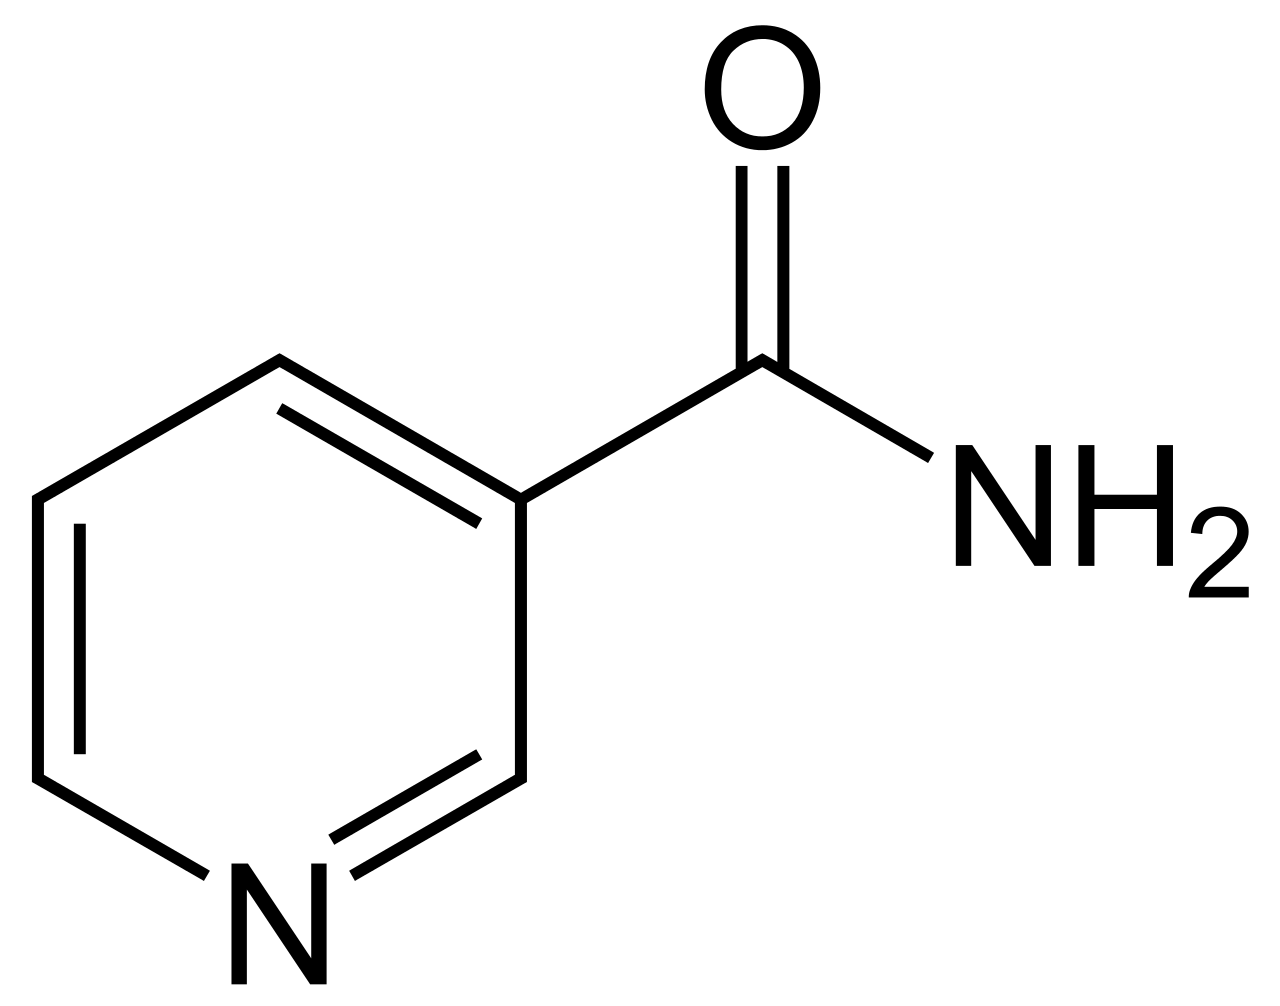
\includegraphics[width=0.5\textwidth]{images/Vitamin_B3_chemical_structure}
\end{figure}

\begin{table}[h]
	\caption{Chemical and physical data}
	\centering \begin{tabular}{| r | l |}
		\hline
		Formula & Smt\\ \hline
		Molar mass & X g$\cdot$mol \textsuperscript{-1}\\ \hline
		Melting point & A--B \degree C (X--Y \degree F)\\ \hline
		Boiling point & A--B \degree C (X--Y \degree F)\\ \hline
		SMILES & \\ \hline
	\end{tabular}
\end{table}
\newpage

\section{About}


\section{Measurement unit}


\section{Dietary recommendations}


\section{Sources}


\chapter{Vitamin B5}
\begin{figure}[h]
	\caption{Chemical structure of Vitamin B5}
	\centering 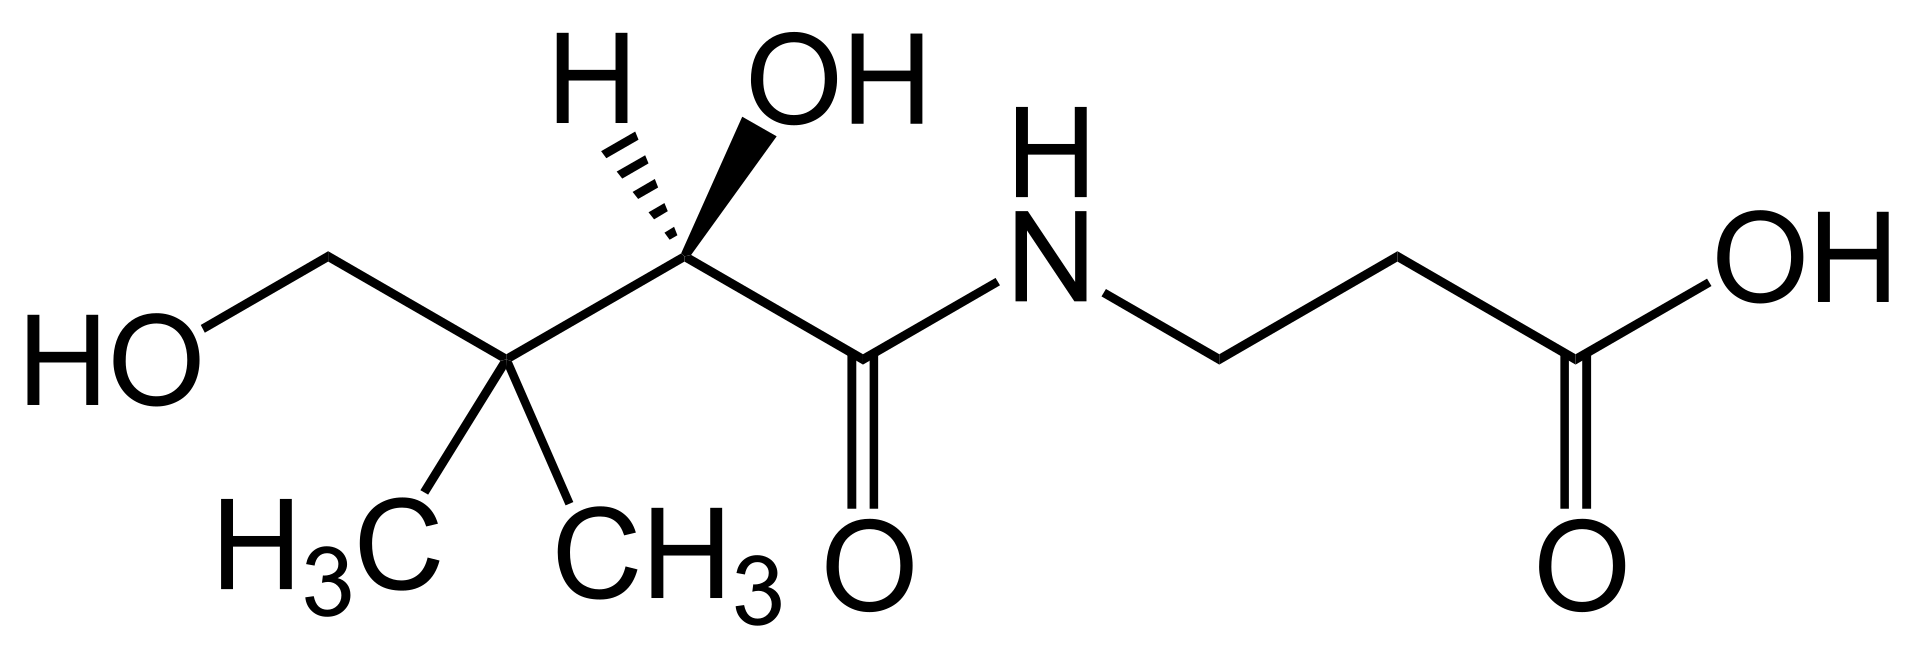
\includegraphics[width=\textwidth]{images/Vitamin_B5_chemical_structure}
\end{figure}

\begin{table}[h]
	\caption{Chemical and physical data}
	\centering \begin{tabular}{| r | l |}
		\hline
		Formula & Smt\\ \hline
		Molar mass & X g$\cdot$mol \textsuperscript{-1}\\ \hline
		Melting point & A--B \degree C (X--Y \degree F)\\ \hline
		Boiling point & A--B \degree C (X--Y \degree F)\\ \hline
		SMILES & \\ \hline
	\end{tabular}
\end{table}
\newpage

\section{About}


\section{Measurement unit}


\section{Dietary recommendations}


\section{Sources}


\chapter{Vitamin B6}
\begin{figure}[h]
	\caption{Chemical structure of Vitamin B6}
	\centering 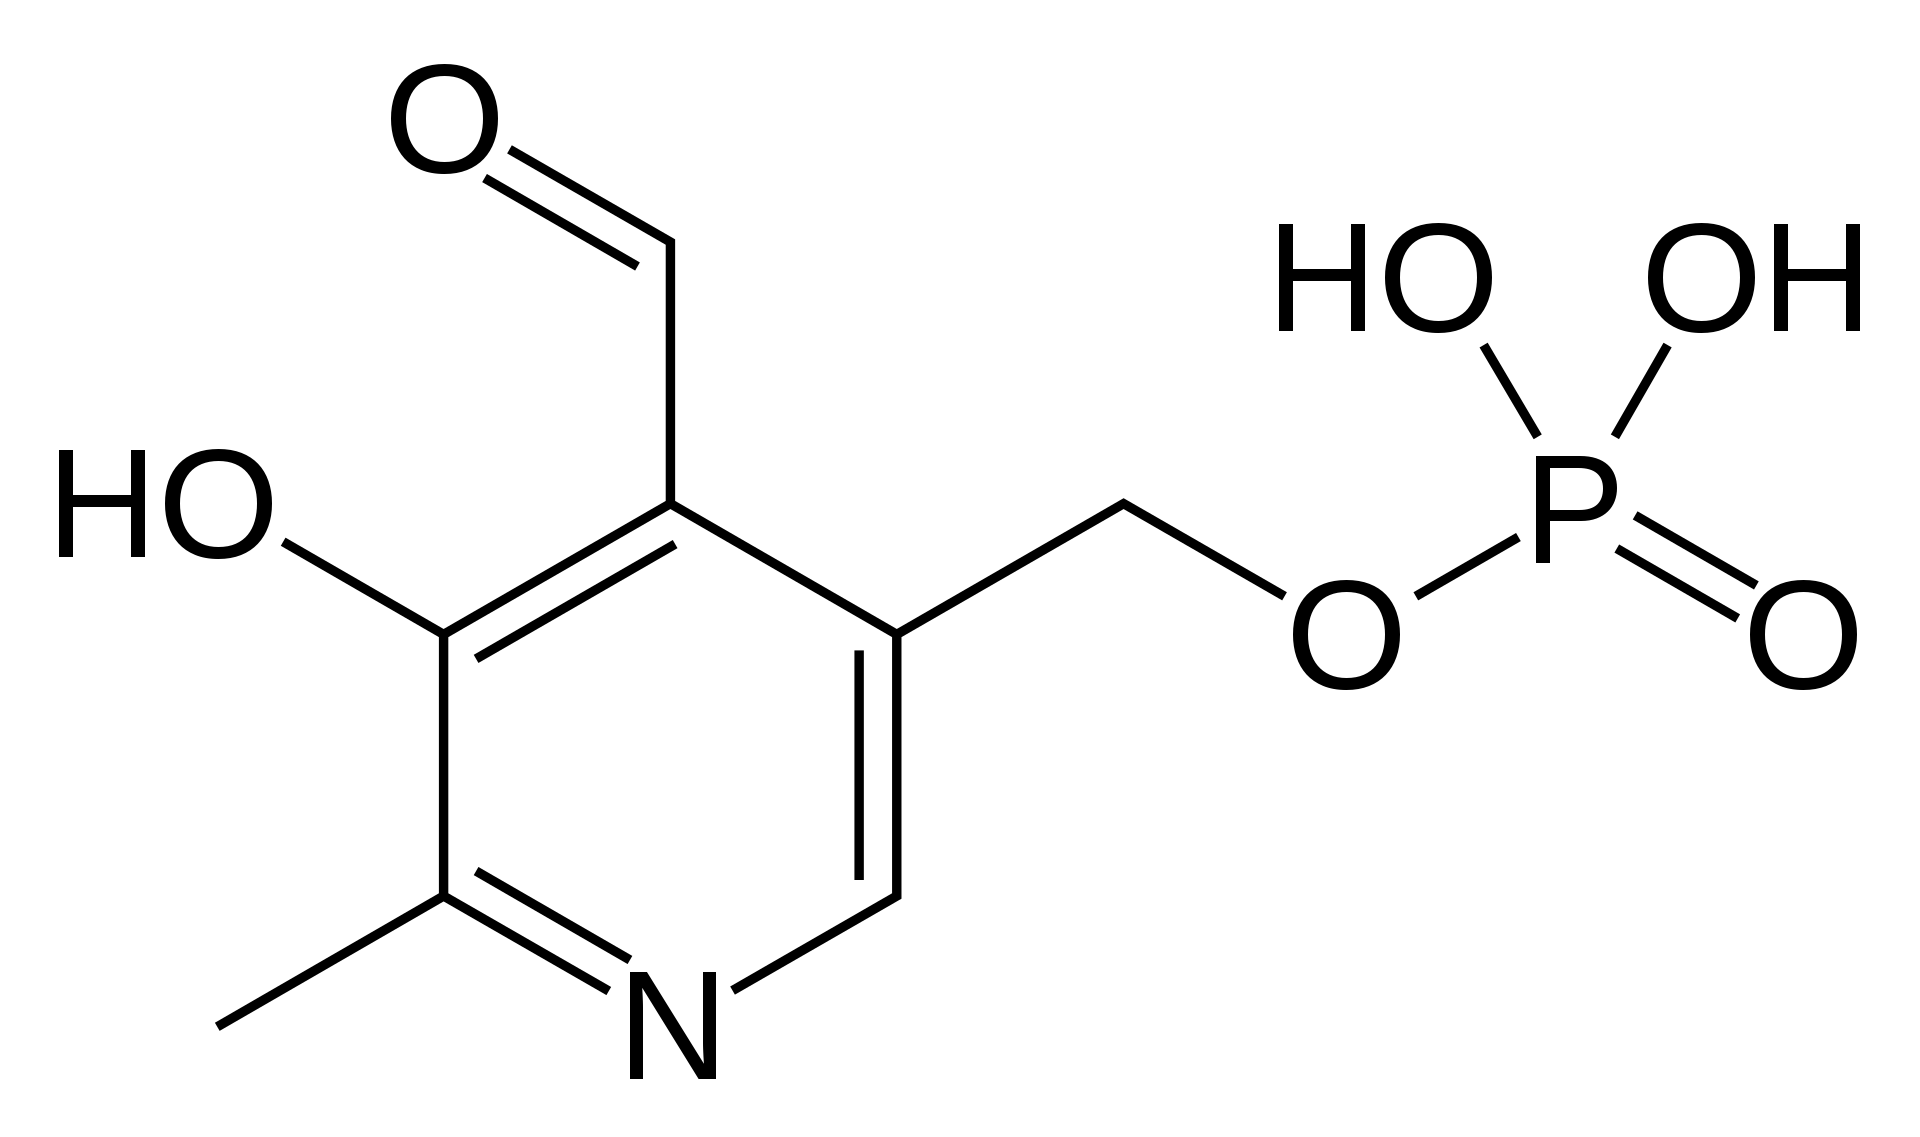
\includegraphics[width=0.75\textwidth]{images/Vitamin_B6_chemical_structure}
\end{figure}

\begin{table}[h]
	\caption{Chemical and physical data}
	\centering \begin{tabular}{| r | l |}
		\hline
		Formula & Smt\\ \hline
		Molar mass & X g$\cdot$mol \textsuperscript{-1}\\ \hline
		Melting point & A--B \degree C (X--Y \degree F)\\ \hline
		Boiling point & A--B \degree C (X--Y \degree F)\\ \hline
		SMILES & \\ \hline
	\end{tabular}
\end{table}
\newpage

\section{About}


\section{Measurement unit}


\section{Dietary recommendations}


\section{Sources}


\chapter{Vitamin B7}
\begin{figure}[h]
	\caption{Chemical structure of Vitamin B7}
	\centering 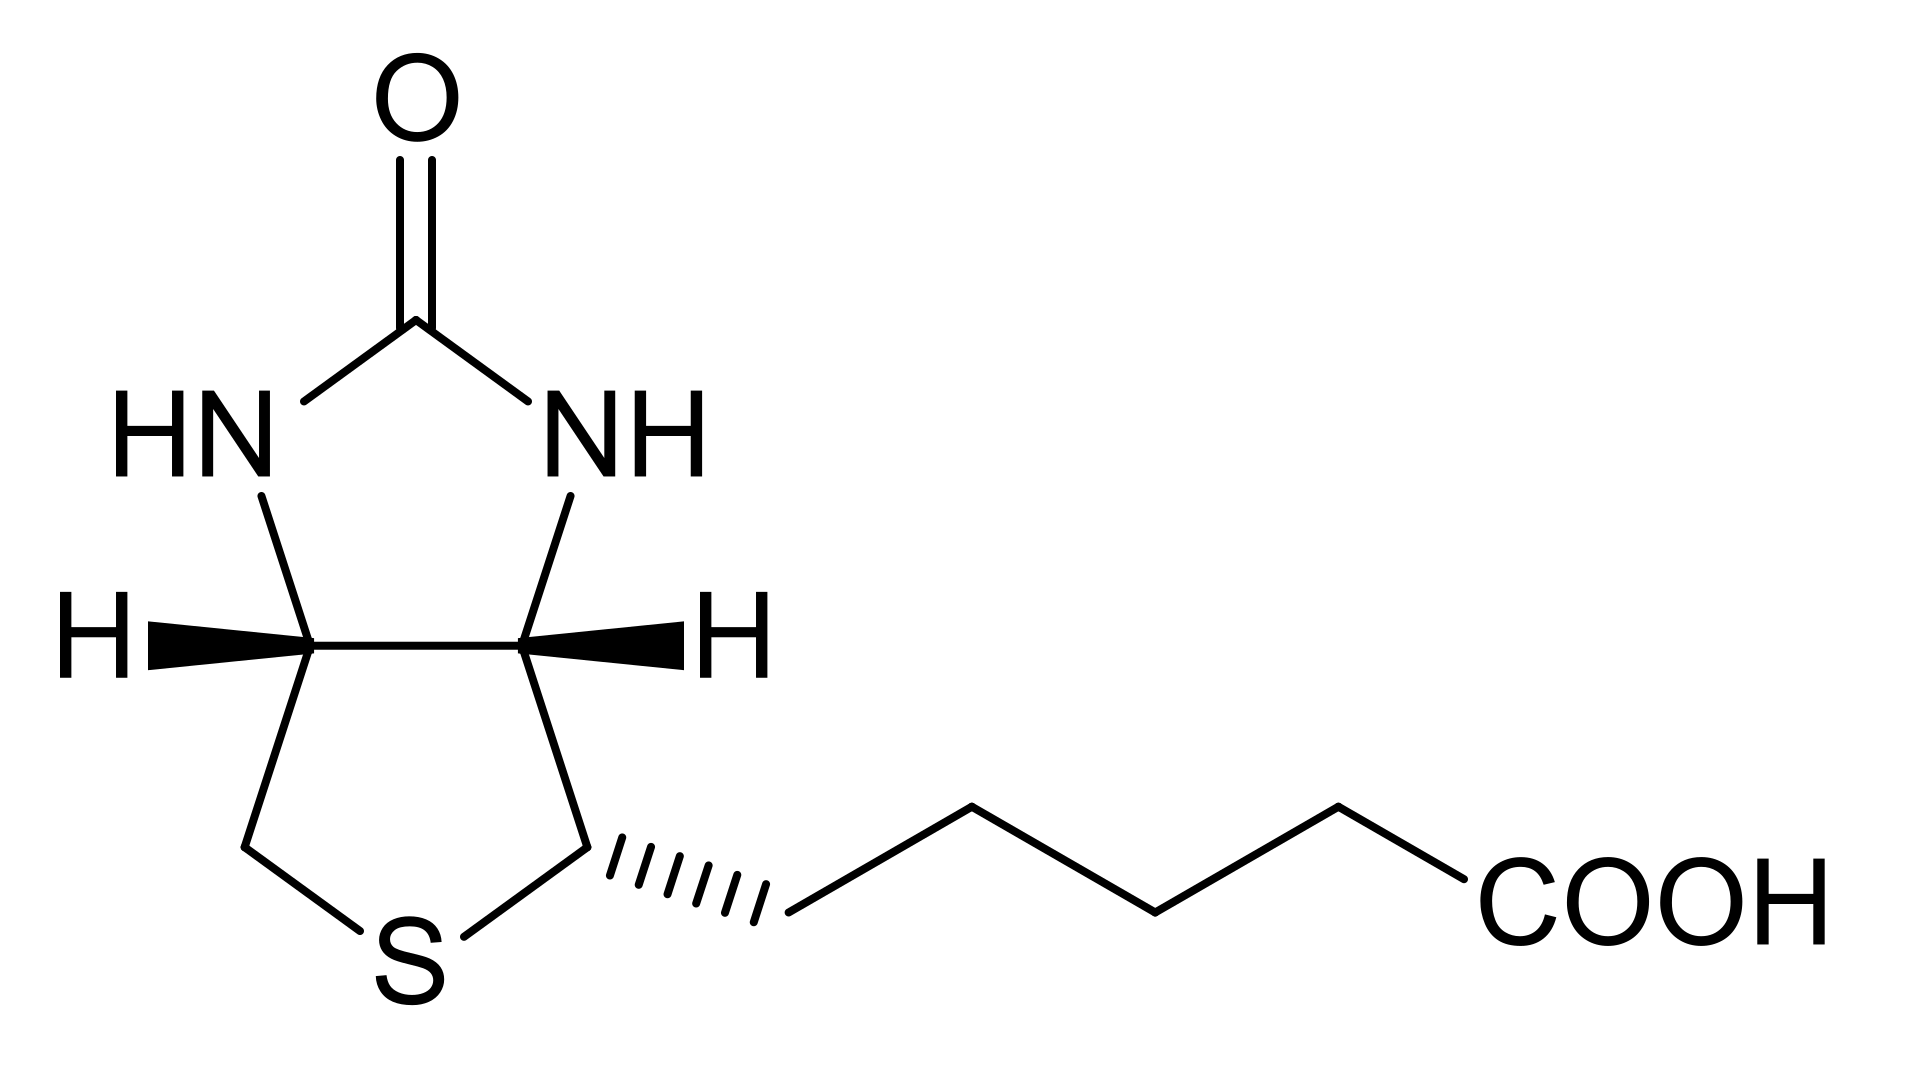
\includegraphics[width=0.75\textwidth]{images/Vitamin_B7_chemical_structure}
\end{figure}

\begin{table}[h]
	\caption{Chemical and physical data}
	\centering \begin{tabular}{| r | l |}
		\hline
		Formula & Smt\\ \hline
		Molar mass & X g$\cdot$mol \textsuperscript{-1}\\ \hline
		Melting point & A--B \degree C (X--Y \degree F)\\ \hline
		Boiling point & A--B \degree C (X--Y \degree F)\\ \hline
		SMILES & \\ \hline
	\end{tabular}
\end{table}
\newpage

\section{About}


\section{Measurement unit}


\section{Dietary recommendations}


\section{Sources}


\chapter{Vitamin B9}
\begin{figure}[h]
	\caption{Chemical structure of Vitamin B9}
	\centering 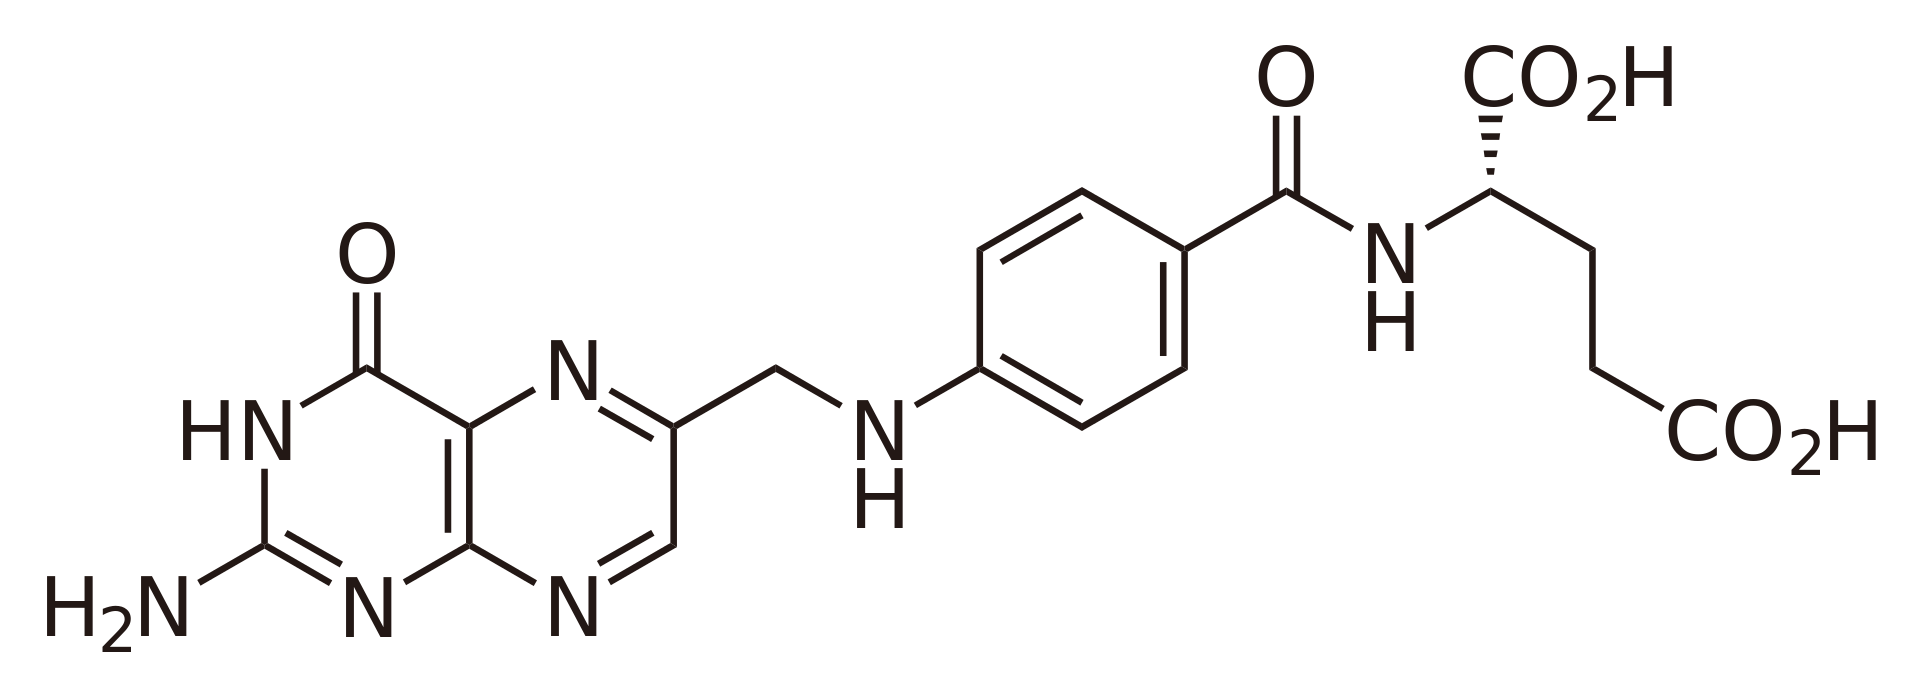
\includegraphics[width=\textwidth]{images/Vitamin_B9_chemical_structure}
\end{figure}

\begin{table}[h]
	\caption{Chemical and physical data}
	\centering \begin{tabular}{| r | l |}
		\hline
		Formula & Smt\\ \hline
		Molar mass & X g$\cdot$mol \textsuperscript{-1}\\ \hline
		Melting point & A--B \degree C (X--Y \degree F)\\ \hline
		Boiling point & A--B \degree C (X--Y \degree F)\\ \hline
		SMILES & \\ \hline
	\end{tabular}
\end{table}
\newpage

\section{About}


\section{Measurement unit}


\section{Dietary recommendations}


\section{Sources}


\chapter{Vitamin B12}
\begin{figure}[h]
	\caption{Chemical structure of Vitamin B12}
	\centering 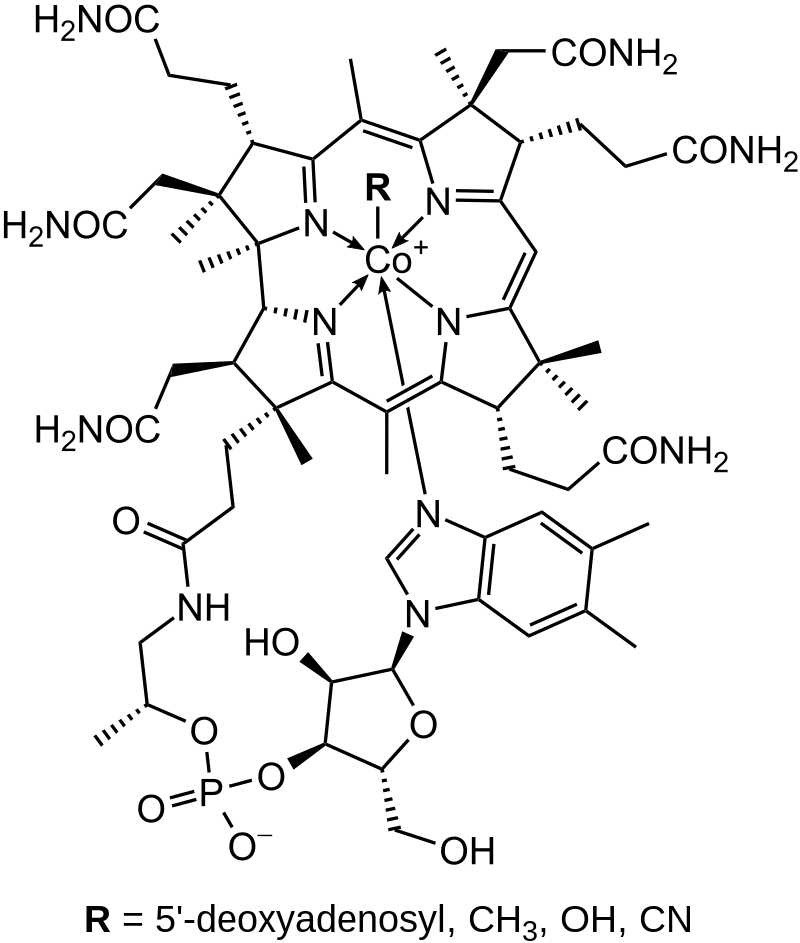
\includegraphics[width=0.5\textwidth]{images/Vitamin_B12_chemical_structure}
\end{figure}

\begin{table}[h]
	\caption{Chemical and physical data}
	\centering \begin{tabular}{| r | l |}
		\hline
		Formula & Smt\\ \hline
		Molar mass & X g$\cdot$mol \textsuperscript{-1}\\ \hline
		Melting point & A--B \degree C (X--Y \degree F)\\ \hline
		Boiling point & A--B \degree C (X--Y \degree F)\\ \hline
		SMILES & \\ \hline
	\end{tabular}
\end{table}
\newpage

\section{About}


\section{Measurement unit}


\section{Dietary recommendations}


\section{Sources}


\chapter{Vitamin C}
\begin{figure}[h]
	\caption{Chemical structure of Vitamin C}
	\centering 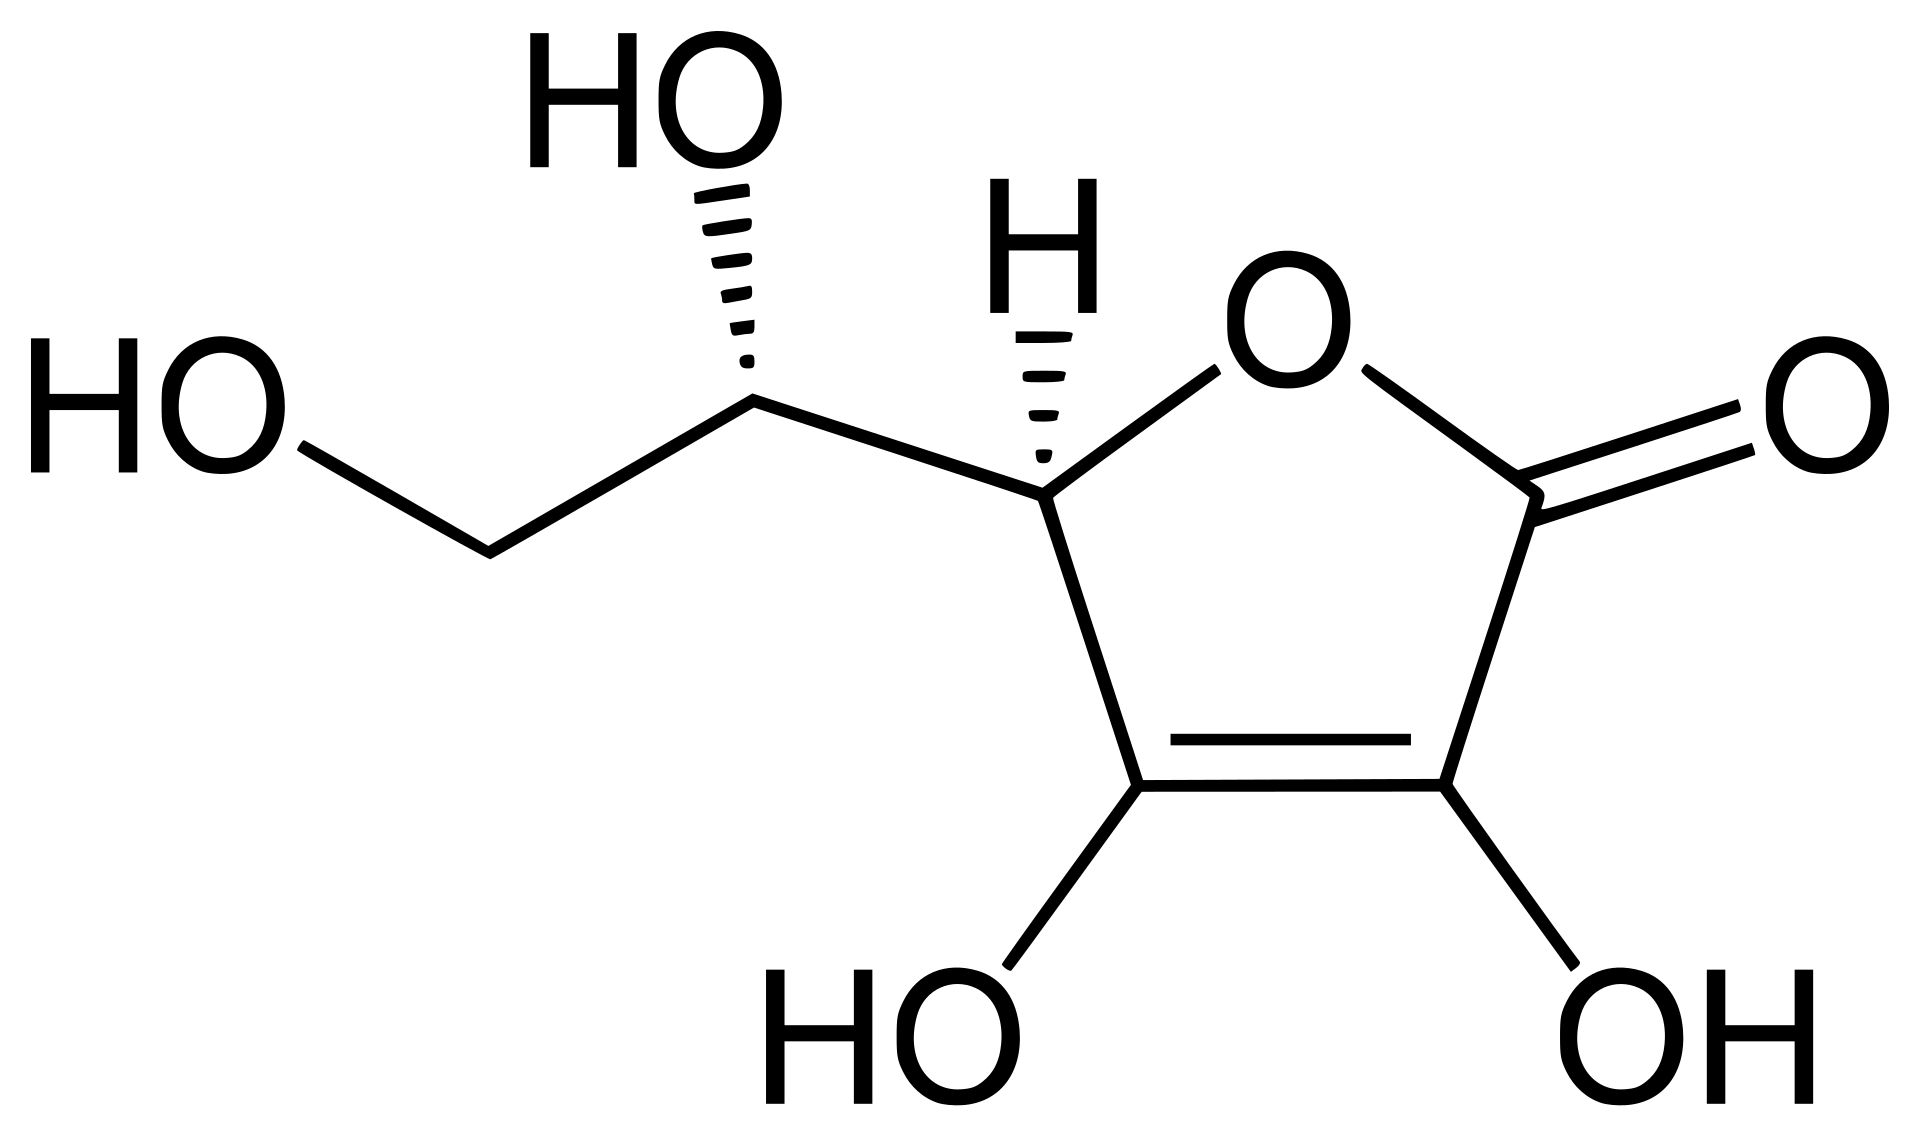
\includegraphics[width=0.75\textwidth]{images/Vitamin_C_chemical_structure}
\end{figure}

\begin{table}[h]
	\caption{Chemical and physical data}
	\centering \begin{tabular}{| r | l |}
		\hline
		Formula & Smt\\ \hline
		Molar mass & X g$\cdot$mol \textsuperscript{-1}\\ \hline
		Melting point & A--B \degree C (X--Y \degree F)\\ \hline
		Boiling point & A--B \degree C (X--Y \degree F)\\ \hline
		SMILES & \\ \hline
	\end{tabular}
\end{table}
\newpage

\section{About}


\section{Measurement unit}


\section{Dietary recommendations}


\section{Sources}


\chapter{Vitamin D}
\begin{figure}[h]
	\caption{Chemical structure of Vitamin D}
	\centering 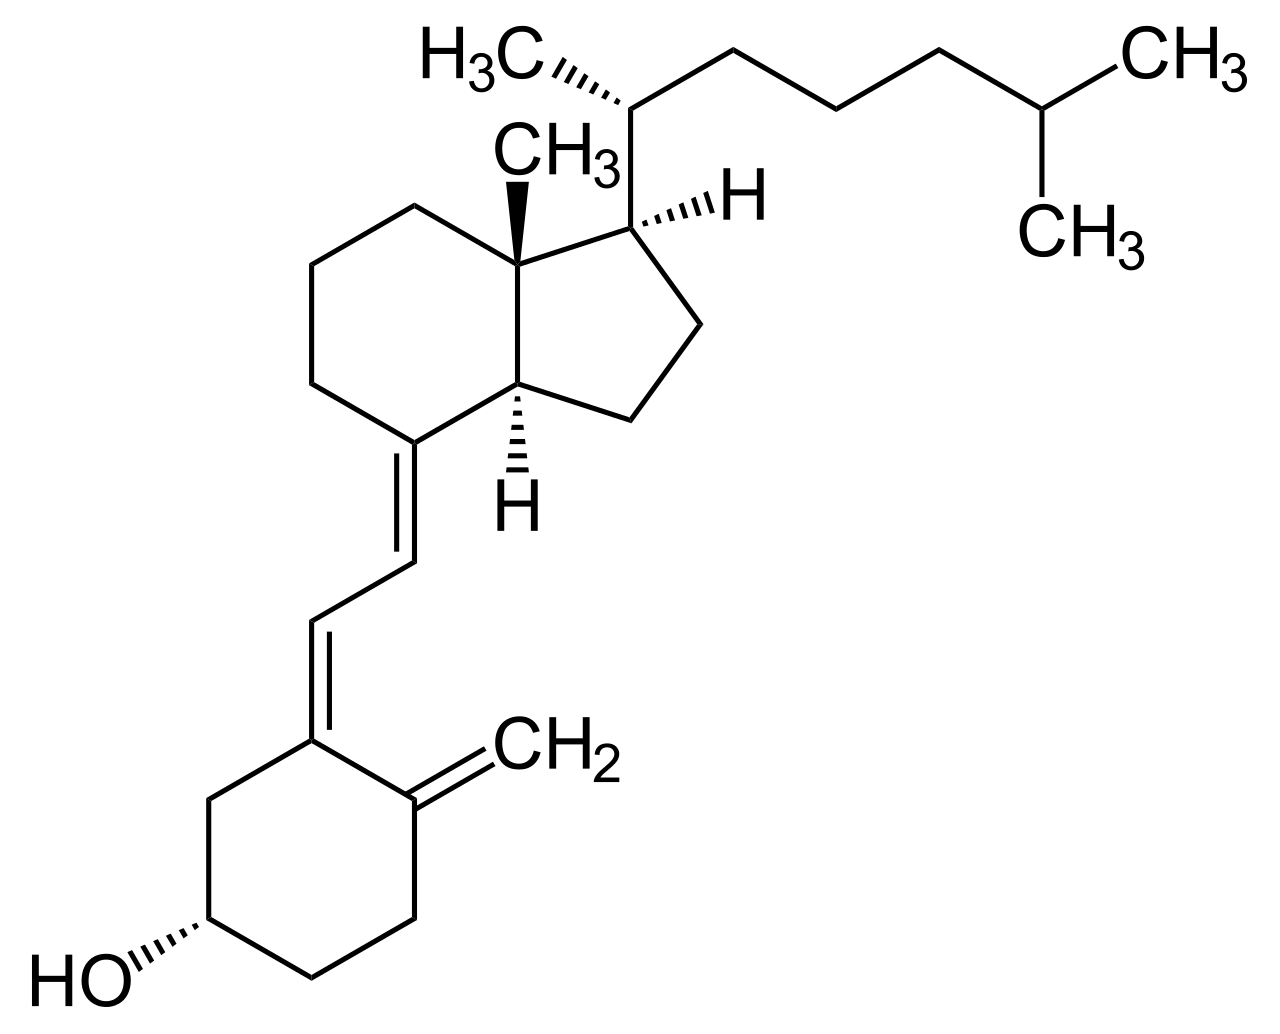
\includegraphics[width=0.75\textwidth]{images/Vitamin_D_chemical_structure}
\end{figure}

\begin{table}[h]
	\caption{Chemical and physical data}
	\centering \begin{tabular}{| r | l |}
		\hline
		Formula & Smt\\ \hline
		Molar mass & X g$\cdot$mol \textsuperscript{-1}\\ \hline
		Melting point & A--B \degree C (X--Y \degree F)\\ \hline
		Boiling point & A--B \degree C (X--Y \degree F)\\ \hline
		SMILES & \\ \hline
	\end{tabular}
\end{table}
\newpage

\section{About}


\section{Measurement unit}


\section{Dietary recommendations}


\section{Sources}


\chapter{Vitamin E}
\begin{figure}[h]
	\caption{Chemical structure of Vitamin E}
	\centering 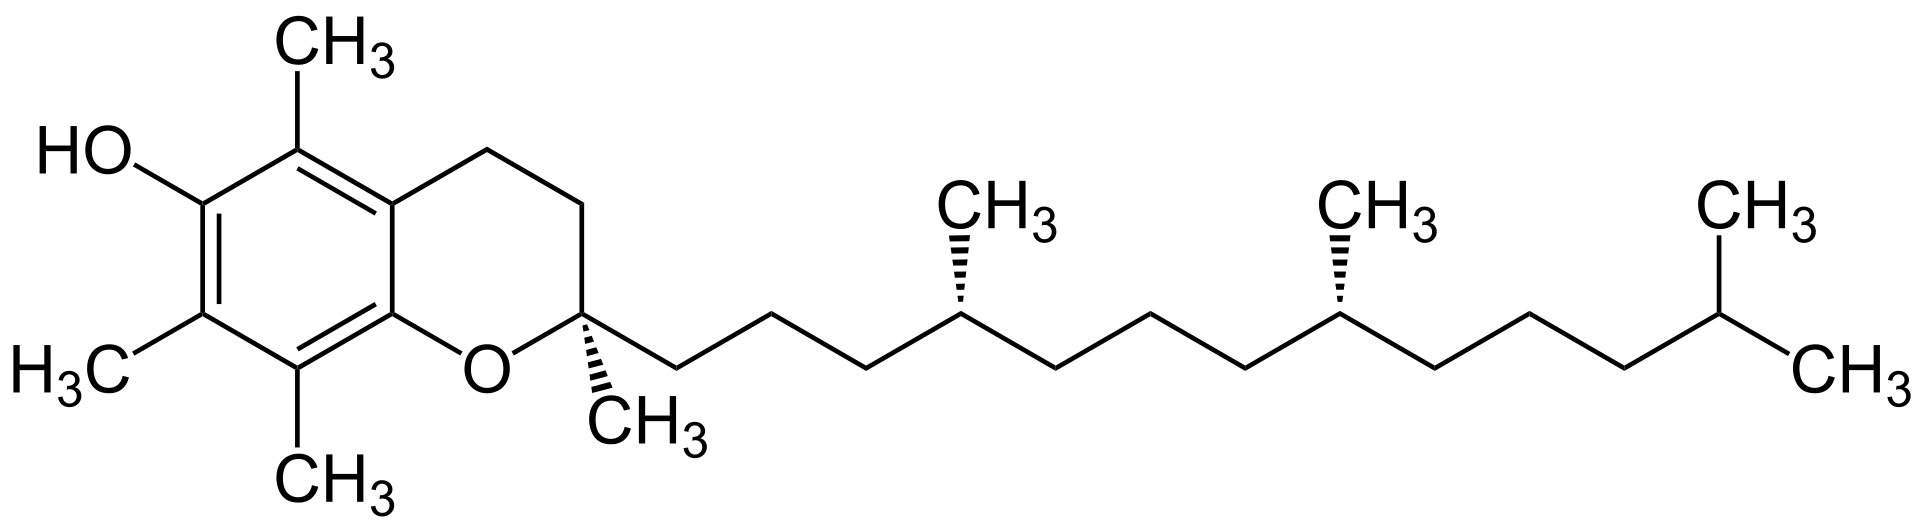
\includegraphics[width=\textwidth]{images/Vitamin_E_chemical_structure}
\end{figure}

\begin{table}[h]
	\caption{Chemical and physical data}
	\centering \begin{tabular}{| r | l |}
		\hline
		Formula & Smt\\ \hline
		Molar mass & X g$\cdot$mol \textsuperscript{-1}\\ \hline
		Melting point & A--B \degree C (X--Y \degree F)\\ \hline
		Boiling point & A--B \degree C (X--Y \degree F)\\ \hline
		SMILES & \\ \hline
	\end{tabular}
\end{table}
\newpage

\section{About}


\section{Measurement unit}


\section{Dietary recommendations}


\section{Sources}


\chapter{Vitamin K1}
\begin{figure}[h]
	\caption{Chemical structure of Vitamin K1}
	\centering 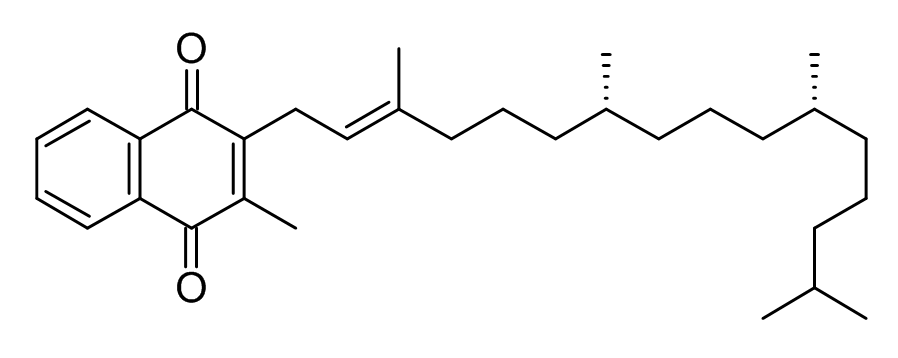
\includegraphics[width=\textwidth]{images/Vitamin_K1_chemical_structure}
\end{figure}

\begin{table}[h]
	\caption{Chemical and physical data}
	\centering \begin{tabular}{| r | l |}
		\hline
		Formula & Smt\\ \hline
		Molar mass & X g$\cdot$mol \textsuperscript{-1}\\ \hline
		Melting point & A--B \degree C (X--Y \degree F)\\ \hline
		Boiling point & A--B \degree C (X--Y \degree F)\\ \hline
		SMILES & \\ \hline
	\end{tabular}
\end{table}
\newpage

\section{About}


\section{Measurement unit}


\section{Dietary recommendations}


\section{Sources}


\chapter{Vitamin K2}
\begin{figure}[h]
	\caption{Chemical structure of Vitamin K2}
	\centering 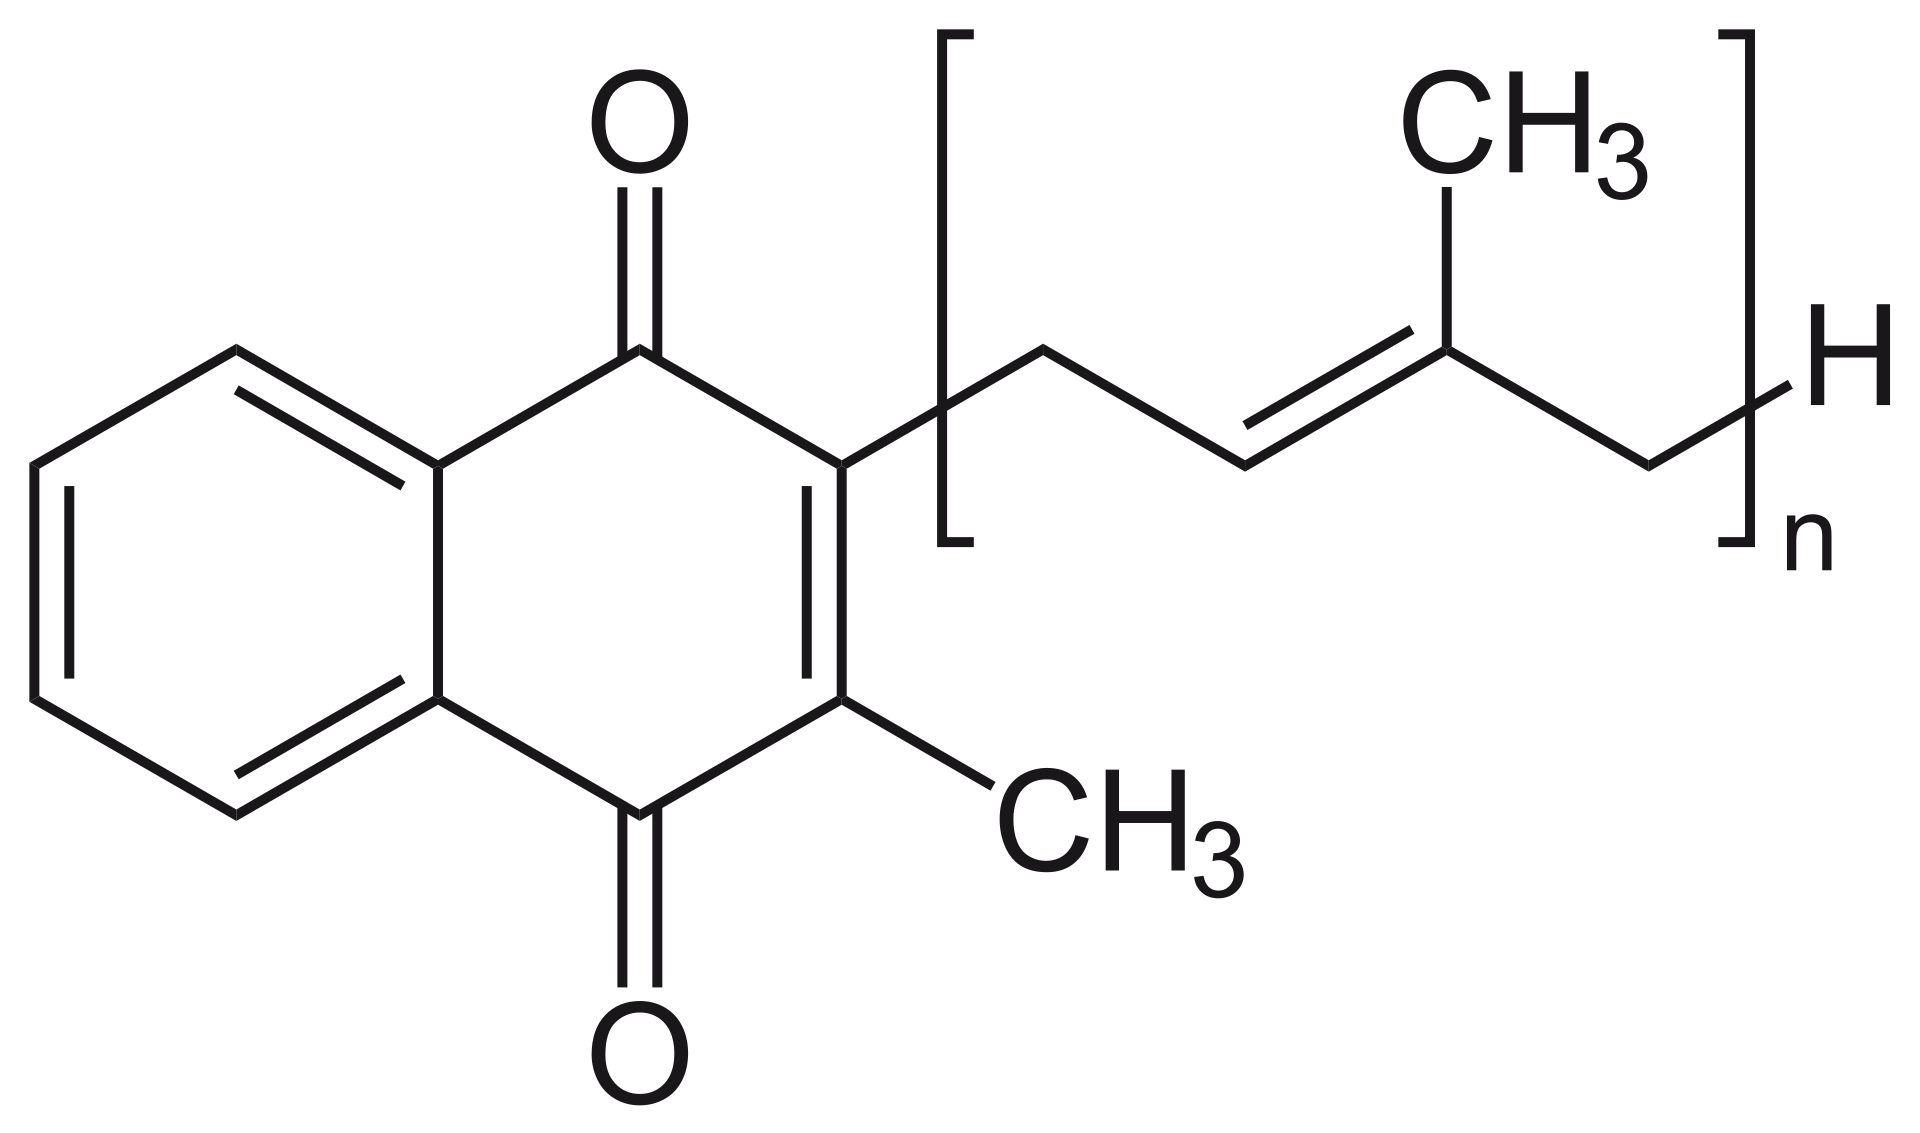
\includegraphics[width=0.75\textwidth]{images/Vitamin_K2_chemical_structure}
\end{figure}

\begin{table}[h]
	\caption{Chemical and physical data}
	\centering \begin{tabular}{| r | l |}
		\hline
		Formula & Smt\\ \hline
		Molar mass & X g$\cdot$mol \textsuperscript{-1}\\ \hline
		Melting point & A--B \degree C (X--Y \degree F)\\ \hline
		Boiling point & A--B \degree C (X--Y \degree F)\\ \hline
		SMILES & \\ \hline
	\end{tabular}
\end{table}
\newpage

\section{About}


\section{Measurement unit}


\section{Dietary recommendations}


\section{Sources}


\chapter{Vitamin K3}
\begin{figure}[h]
	\caption{Chemical structure of Vitamin K3}
	\centering 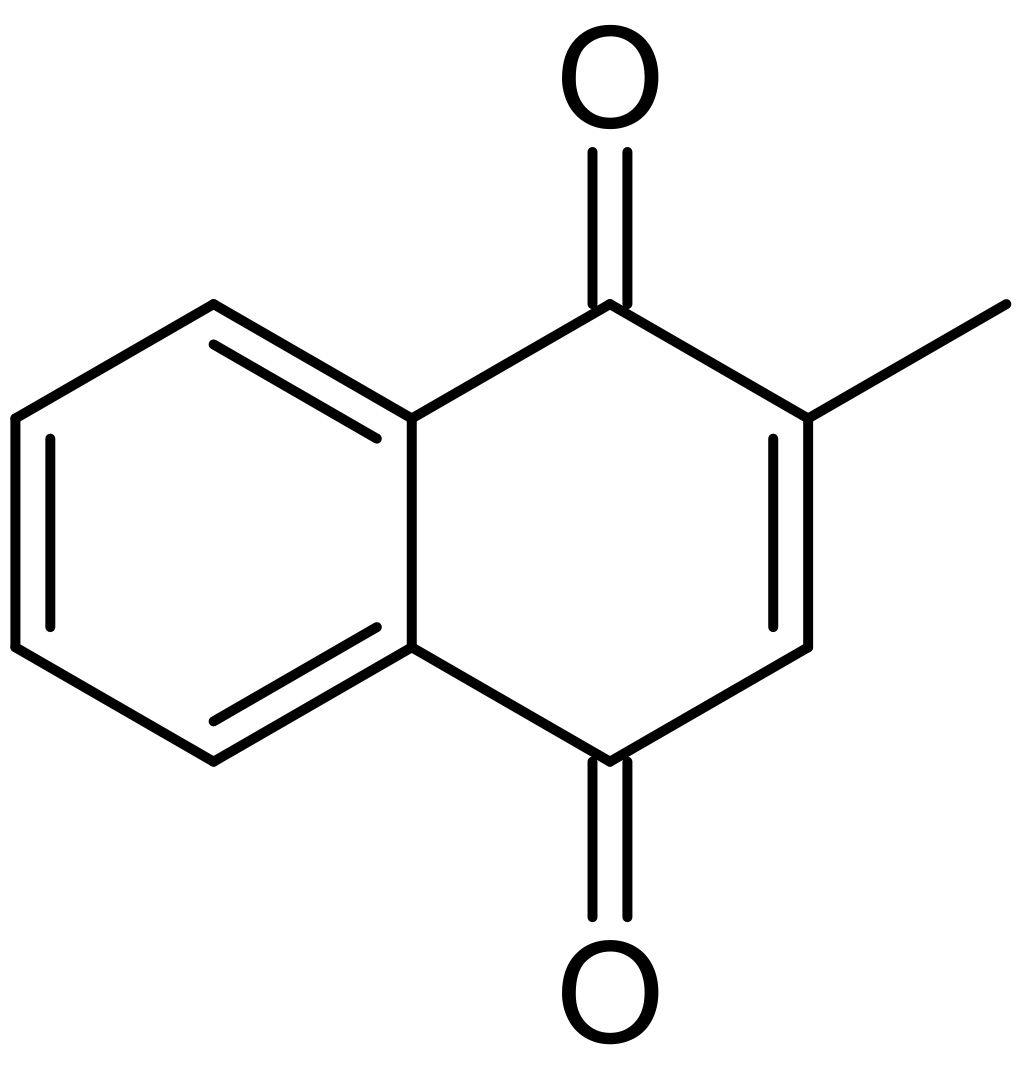
\includegraphics[width=0.5\textwidth]{images/Vitamin_K3_chemical_structure}
\end{figure}

\begin{table}[h]
	\caption{Chemical and physical data}
	\centering \begin{tabular}{| r | l |}
		\hline
		Formula & Smt\\ \hline
		Molar mass & X g$\cdot$mol \textsuperscript{-1}\\ \hline
		Melting point & A--B \degree C (X--Y \degree F)\\ \hline
		Boiling point & A--B \degree C (X--Y \degree F)\\ \hline
		SMILES & \\ \hline
	\end{tabular}
\end{table}
\newpage

\section{About}


\section{Measurement unit}


\section{Dietary recommendations}


\section{Sources}


\chapter{Choline}
\begin{figure}[h]
	\caption{Chemical structure of Choline}
	\centering 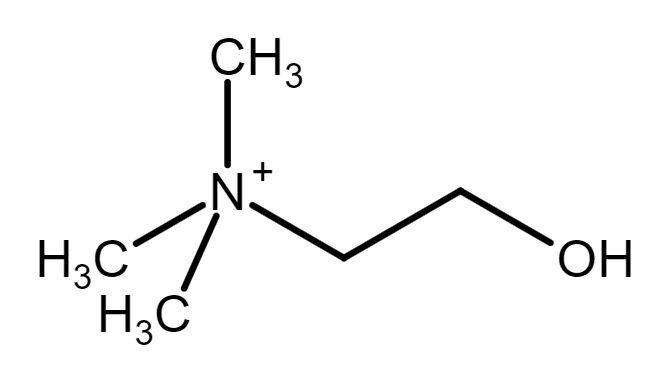
\includegraphics[width=0.75\textwidth]{images/Choline_chemical_structure}
\end{figure}

\begin{table}[h]
	\caption{Chemical and physical data}
	\centering \begin{tabular}{| r | l |}
		\hline
		Formula & Smt\\ \hline
		Molar mass & X g$\cdot$mol \textsuperscript{-1}\\ \hline
		Melting point & A--B \degree C (X--Y \degree F)\\ \hline
		Boiling point & A--B \degree C (X--Y \degree F)\\ \hline
		SMILES & \\ \hline
	\end{tabular}
\end{table}
\newpage

\section{About}


\section{Measurement unit}


\section{Dietary recommendations}


\section{Sources}


\listoffigures


\listoftables


\end{document}